\imgchapter[left]{8cm}{chapter_6_title}{Análise Sobre Abstrações de Processos}
\label{cap:analise-sobre-abstracoes-de-processos}

No Capítulo \ref{cap:trabalhos-analisados}, introduzimos os principais trabalhos
que orbitam em torno de novas abstrações de processos e, a partir de tais
pesquisas, pretendemos desenvolver neste capítulo uma reflexão sobre suas principais
características. Para isso, realizamos diversas análises sobre o estado da arte
da pesquisa em processos e apresentamos um modelo teórico que visa fornecer
uma perspectiva para a nova geração de abstrações de processos. Como resultado,
responderemos as seguintes questões de pesquisa:

\begin{quote}
 \item \textit{QP1:.} ``Quais são as características desejáveis para a próxima geração de abstrações de processos?''
 \item \textit{QP2:.} ``Quais são os principais desafios em se implementar a próxima geração de abstrações de processos?''
\end{quote}

Este trabalho se diferencia dos trabalhos apresentados no
Capítulo~\ref{cap:trabalhos-analisados} por buscar uma visão unificada sobre as
novas extensões nas abstrações de processos e por levar em conta SOs de uso
cotidiano, em especial o GNU/Linux. Esse último critério torna-se relevante
para futuras investigações na área, uma vez que, se tais abstrações alcançarem
SOs de ampla utilização, o impacto e o crescimento da área serão significativos.

\section{Potenciais e Dificuldades Para a Adoção de Novas Abstrações de Processos}
\label{sec:potenciais}
%TODO: Ver a onde da para cortar
Quando a academia faz uma nova proposta para sistemas que estão no ``estado da
prática'', ela deve ser genérica o bastante para ser utilizada por
múltiplas linguagens de programação e deve também considerar questões
referentes a compatibilidade, melhor uso do hardware disponível e
confiabilidade. Assim, apesar dos avanços trazidos pelas pesquisas em SO, elas
estão limitadas às diferentes restrições existentes nos SOs utilizados tanto em
produção quanto em projetos de pesquisa.

SOs usados em produção demandam rigorosa validação para manter o sistema
estável em uma variedade de configurações. Espera-se que um SO maduro busque
prevenir acessos ilegais à memória, impossibilitar a violação de APIs, evitar
consumo excessivo de recursos e impedir erros de sincronização ou
\textit{locking}. Essas características precisam ser garantidas pelo SO
\citep{mondrix}, porém, como esperado, tais restrições dificilmente são
atendidas por propostas de pesquisas devido ao foco dos pesquisadores
em um único problema, desconsiderando assim outros impactos. Por esse motivo,
para que um novo componente sugerido a partir de uma pesquisa acadêmica chegue
aos SOs atuais, é importante garantir que as aplicações que já existem não
sofram impactos negativos em termos de desempenho e de uso.

Outra perspectiva que deve ser considerada é o contínuo desenvolvimento de novos
recursos de hardware. Por exemplo, frequentemente observam-se componentes que
são especializados em um nicho e que, ao longo do tempo, chegam ao usuário
final, tornando-se comuns. Um caso simples que ilustra tal evolução é o
uso de hardware especializado para virtualização, uma vez que esses existiam
apenas para servidores e hoje estão disponíveis para a maioria dos usuários
comuns. Tais recursos representam um novo leque de opções não exploradas,
inclusive possíveis melhorias para as atuais abstrações de processos.

Entretanto, para incorporar novos recursos de hardware à abstração de processos,
não se deve descartar que tal recurso pode não estar disponível para alguns
usuários. Por essa razão, qualquer mudança nos processos para adicionar suporte
a novos recursos de hardware deve levar em consideração todo tipo de situação.
De modo inverso, propostas para melhorar uma abstração de processos podem
sugerir mudanças no hardware e promover avanços no estado da arte dos chips
modernos. Claro que a evolução do hardware necessita de cautela para evitar
quebra de compatibilidade binária com aplicações legadas. Infelizmente, é
preciso ter em mente que as alterações de hardware e suas limitações fazem com
que propostas que dependem de tal evolução sejam difíceis de serem adotadas, e
tornam a ampla adoção de uma determinada melhoria às vezes impraticável.

Algumas das novas abstrações de processos propostas por pesquisadores têm
enorme dependência com outras tecnologias experimentais. Se, por um lado, isso
traz vantagens para as tecnologias em desenvolvimento, por outro, reduz a chance
de adoção de uma nova abstração de processos por um SO de produção devido à
dependência dessa abstração de tecnologias instáveis.

Encontrar um bom balanceamento entre academia e indústria de forma a levar
benefícios para os usuários não é uma tarefa trivial. Nesse sentido, novas
propostas de mudanças na abstração de processos devem considerar as limitações
citadas nessa seção para que possam atender aos requisitos de qualidade
exigidos pelos SOs de uso cotidiano. Infelizmente, afirmar que uma proposta da
academia pode ser adotada ou não pela indústria é uma tarefa complexa dada a
enorme quantidade de variáveis envolvidas em tal análise. Mesmo assim, para
posicionar o leitor em termos do estado da arte e da prática, buscamos
estabelecer um ``potencial de adoção'' de uma nova proposta. Com base nos
critérios apresentados, definimos um conjunto de variáveis que auxilie
na definição das chances de uma pesquisa ser adotada pela indústria:

\begin{enumerate}
  \item
\textbf{Dependência Técnica}: indica se o trabalho é construído
levando-se em consideração outras tecnologias não estabilizadas. Consideramos
tal aspecto um problema para a adoção da nova técnica.

  \item \textbf{Dependência de Compatibilidade}: refere-se às propostas que
exigem alterações na semântica das aplicações em espaço de usuário para que
elas possam tirar proveito de alguma melhoria.

  \item
\textbf{Dependência de Compilador}: propostas que dependem de alterações no
compilador. Nesses casos, consideramos que a adoção torna-se mais complicada
uma vez que dois projetos precisam ser alterados.

  \item
\textbf{Implementação Pesada}: consideramos as implementações pesadas mais
complicadas, uma vez que necessitam realizar mudanças no núcleo do SO, o que
dificulta a adoção.

  \item
\textbf{Implementação Independente}: refere-se a propostas de novas
implementações, claramente de difícil adoção.

  \item
\textbf{Hardware Novo}: indica que a proposta depende de um
hardware novo que só existe em algum contexto específico ou mesmo que ainda não
foi implementado.

  \item
\textbf{Característica Específica de Hardware}: refere-se a propostas de
utilização de algum hardware bem consolidado para algum propósito diferente do
original.

\end{enumerate}

A Tabela \ref{tab:adocao} tenta apresentar o potencial de adoção de cada uma
das propostas citadas no Capítulo \ref{cap:trabalhos-analisados} de acordo com
as variáveis discutidas nesta seção. Na tabela, temos uma marcação indicada
pelo simbolo \ding{54} que significa que uma determinada proposta possui a
limitação indicada na coluna correspondente. Se a proposta não contém tal restrição, então ela
é marcada com o simbolo \ding{52}. Por uma questão de simplicidade, para
definir o potencial de adoção, atribuímos zero para cada \ding{54} e um para
\ding{52}. Por fim, toda vez que a opção ``Hardware Novo'' é marcada,
consideramos que a proposta também requer características específicas de
hardware; para as variáveis referentes à implementação, consideramos que quando
uma proposta parte de uma implementação independente, ela também é considerada
pesada.

\begin{table}[]
\small
\centering

\begin{tabular}{|@{}c@{}|@{}c@{}|@{}c@{}|@{}c@{}|@{}c@{}|@{}c@{}|@{}c|c@{}|@{}c@{}|}
% HEADERS
\hline
  \multirow{2}{*}{Trabalho}          &
  \multicolumn{3}{c|}{Dependência}   &
  \multicolumn{2}{c|}{Implementação} &
  \multicolumn{2}{c|}{Hardware}       &
  \multirow{2}{*}{Adoção} \\ \cline{2-8} &
      Técnica & Compatibilidade & Compilador & Pesada & Independente &
      \multicolumn{1}{c|}{Novo} & Característica &
\\ \hline
%           Técnica     Compatib    Compilaca   Pesada      Independente                     Novo        Caracact   Adocao
Dune      & \ding{54} & \ding{54} & \ding{54} & \ding{54} & \multicolumn{1}{c|}{\ding{54}} & \ding{54} & \ding{52} & \\ \hline
Shreds    & -- & -- & -- & \ding{54} & \multicolumn{1}{c|}{--} & -- & -- & \\ \hline
Wedge     & \ding{54} & \ding{52} & \ding{52} & \ding{52} & \multicolumn{1}{c|}{\ding{54}} & \ding{54} & \ding{54} & \\ \hline
\begin{tabular}[c]{@{}c@{}}Resource\\ Container\end{tabular} & & & & & \multicolumn{1}{c|}{} & & & \\ \hline
Nooks     & \ding{54} & \ding{52} & \ding{54} & \ding{52} & \multicolumn{1}{c|}{\ding{54}} & \ding{54} & \ding{54} & \\ \hline
Mondrian  & -- & -- & -- & -- & \multicolumn{1}{c|}{ -- } & -- & -- & \\ \hline
SpaceJMP  & \ding{54} & \ding{52} & \ding{52} & \ding{52} & \multicolumn{1}{c|}{\ding{54}} & \ding{54} & \ding{54} & \\ \hline
LwC       & \ding{54} & \ding{52} & \ding{54} & \ding{52} & \multicolumn{1}{c|}{\ding{54}} & \ding{54} & \ding{54} & \\ \hline
Exokernel & -- & -- & -- & -- & \multicolumn{1}{c|}{--} & -- & -- & \\ \hline
\end{tabular}

\caption{Potencial de adoção}
\label{tab:adocao}

\end{table}


\section{Extração de Conceitos Derivados das Pesquisas em Abstrações de Processos}
\label{sec:extracao}

Todas as pesquisas apresentadas no Capítulo \ref{cap:trabalhos-analisados}
configuram o estado da arte no que se refere às abstrações de processos.
Infelizmente, nenhuma delas encontra-se no código principal de qualquer SO de
uso cotidiano. Parte desse problema vem dos fatos apresentados anteriormente na Seção
\ref{sec:potenciais}, contudo outros aspectos que contribuem para que tais
propostas não estejam presentes nos SO modernos vêm da falta de unificação e
sistematização de tais ideias. Ao analisar cada uma das propostas, notamos que
todas elas propõem direta ou indiretamente algum nível de desacoplamento entre
os elementos presentes no SO. Tal observação nasce da abordagem radical tomada
pelos criadores do Exokernel, que levaram o nível de desacoplamento do SO ao
extremo. Apesar do Exokernel ser um sistema de difícil adoção em termos
práticos, ele nos alerta sobre as vantagens da redução de dependências
entre os elementos do SO e as possibilidades que ela pode levar ao espaço de
usuário. Tendo isso em mente, revisitamos de forma breve alguns dos trabalhos
apresentados no Capítulo \ref{cap:trabalhos-analisados} sob a ótica do
desacoplamento e seus potenciais benefícios.

Iniciamos analisando o projeto Dune. Esse projeto traz uma nova perspectiva de uso dos recursos de virtualização
disponibilizados pelas CPUs modernas que, consequentemente, traz dois
benefícios diretos: otimização e flexibilidade. Ao utilizar os recursos de
virtualização para acelerar certas tarefas, o Dune promoveu avanços em um setor
difícil de ser otimizado. Além disso, tais melhorias facilitam certas
implementações no espaço de usuário, pois removem a necessidade de códigos com
técnicas avançadas que visam trazer melhorias de desempenho; em outras
palavras, a proposta do Dune pode melhorar a legibilidade de alguns códigos.
Os avanços citados foram factíveis graças ao \textbf{desacoplamento da
virtualização}, que possibilita entregar melhorias de desempenho no
espaço de usuário de maneira relativamente simples (do ponto de vista da
aplicação) e também fornece ganhos de segurança.

Já o projeto Nooks se distancia um pouco da abstração de processos, uma vez que
busca tornar o núcleo do SO mais resiliente. Contudo, ao criar mecanismos
que reagem de forma a reduzir as chances de o sistema quebrar, tal proposta
apresenta o \textbf{desacoplamento dos recursos}, de forma a fornecer mecanismos
para que os processos possam se recuperar ou tomar ações em casos de falhas.
Adicionalmente, essa técnica cria um interessante mecanismo de
comunicação entre as extensões do Kernel e os seus drivers, permitindo que o SO
se ``defenda'' de problemas que ocorram com um código que foi acoplado ao seu
núcleo.

De forma mais direta e sistemática, o \textit{Resource Container} sugere o
controle fino do gerenciamento de recursos e consequentemente o
\textbf{desacoplamento do gerenciamento de recursos} de tal elemento. De certa
maneira, essa proposta já pode ser encontrada incorporada nos SOs atuais, sob a
forma de contêineres no Linux, mais especificamente, como o
\textit{cgroups}\footnote{\emph{cgroups} é uma funcionalidade fornecida pelo
Linux que permite limitar e isolar recursos de uma coleção de processos.}. A
principal contribuição do do \emph{Resource Container} vem da sua capacidade de permitir que a
própria aplicação tome conta da sua execução.  Ainda que parte das ideias
apresentadas por esse trabalho estejam presentes em alguns SOs, as
implementações ainda são relativamente reduzidas em termos do escopo
apresentado na pesquisa.

Uma abordagem alternativa que visa atender uma nova geração de computadores com
memórias não voláteis na ordem dos petabytes é o SpaceJMP/MVAS.  Os autores
sugerem o \textbf{desacoplamento do VAS dos processos} e permitir que eles tenham
múltiplos VAS e, de forma reativa, a aplicação torne-se capaz de mudar o VAS
atual. Essa abordagem faz com que um processo consiga acessar regiões muito
maiores do que aquelas garantidas pelo tamanho de um VAS. Indiretamente,
desacoplar um VAS adiciona a possibilidade de criar processos persistentes,
isto é, que vivem mesmo após o reboot ou mesmo após um problema. Desacoplar o VAS
pode trazer benefícios para aplicações de \textit{checkpoints}, melhorar o
gerenciamento de bibliotecas, e elevar o nível de isolamento e compartilhamento.

O projeto  Light-weight Context (lwC) indiretamente propõe o total
\textbf{desacoplamento do PC}; vale observar que os autores explicitam outros
desacoplamentos, contudo, para esse trabalho, acreditamos que o desacoplamento
do PC é o que melhor descreve as inovações propostas. Desacoplar o PC leva uma
infinidade de possibilidades para o espaço de usuário, uma vez que o processo
pode fazer operações semelhantes às do escalonador sem grandes custos e dentro
do mesmo intervalo de execução do processo. lwC tem como principal
característica um robusto e interessante modelo de programação que permite
às aplicações no espaço de usuário utilizarem novos paradigmas de desenvolvimento.
Isso cria diversas oportunidades para desenvolver novos tipos de manipulações,
tal como criar \emph{snapshots} do estado atual do processo e depois reverter o
processo para o estado anterior. Dado os múltiplos \emph{snapshots}
(contextos), é possível fazer com que um processo em execução mude para uma
outro contexto com diferentes restrições de acesso a memória permitindo isolar
trechos de código sensível.  Ao contrário do que parece, isso não é como
utilizar \emph{threads} ou processos independentes. Por não haver dependência
do escalonador para mudar o contexto do processo (o que é razoavelmente caro),
a própria aplicação pode escolher quando e qual contexto manipular e fornecer,
assim, um controle fino para os programadores (o que pode melhorar o desempenho
e a segurança).

De modo geral, percebemos que vários dos trabalhos analisados têm preocupação com o gerenciamento e acesso a
memória; em especial, vários deles questionam o tratamento dado à memória pelos
SOs atuais.  A abordagem de utilizar um único espaço de endereçamento por
processo tem se provado eficiente ao longo dos anos, porém, apesar do seu
sucesso, essa não é uma abordagem à prova de falhas e ainda carece de
melhorias. Primeiramente, a abordagem de isolar os processos por meio do
espaço de endereçamento linear melhora a confiabilidade do sistema e a
segurança. Entretanto, um processo não tem uma forma de restringir o seu próprio
acesso ao seu segmento de memória, o que pode ser útil para reduzir os riscos de
falhas de segurança ocasionados por binários de terceiros. Em segundo lugar, o
controle do compartilhamento de memória acontece no tamanho de uma página e
cria a oportunidade para explorar falhas, tais quais \emph{buffer e stack
overflow} ou mesmo o compartilhamento de bibliotecas comprometidas. Com essa preocupação, os
trabalhos Wedge, shreds e mondrix/mondrian buscam trazer melhorias para essas fragilidades.

Analisando as abstrações de processos da perspectiva da segurança, o projeto
Wedge retoma uma antiga premissa que defende o princípio do menor privilégio.
Ela afirma que precisamos mudar a lógica atual de conceder permissão por
padrão para uma ideia de negar permissão por padrão. Essa mudança de paradigma
torna supostamente possível a redução das chances de ataques e vazamento de
dados, uma vez que o programador precisa indicar explicitamente o que será
exposto. Tal pesquisa indiretamente propõe o \textbf{desacoplamento dos
privilégios} da abstração de processos. Além disso, ela mantém a
compatibilidade entre aplicações novas e legadas, sendo uma opção de uso ao programador.

Entrando um pouco mais nas questões de proteção e controle-fino da memória,
destacamos o shreds e o mondrix/mondrian. shreds nasce com a ideia de evitar
ataques conhecidos como abusos intra-processos de conteúdo da memória. Os
autores defendem que o acesso a certas regiões da memória de um processo
que esteja executando em espaço de usuário merecem proteção especial. Em tal proposta, os
autores utilizaram um recurso específico dos processadores ARM em conjunto com
um mecanismo de gerenciamento da região de memória (Seção
\ref{sec:outros_mecanismos_memoria}). Essa proposta entrega mais flexibilidade,
segurança e controle ao acesso da memória.

Na mesma linha de fornecer controle fino sobre a memória, os autores do Mondrix
propuseram, de forma mais radical, um mecanismo de controle do acesso à memória
no nível das palavras de dados. Para isso, os autores sugerem alterações no
hardware e no SO de forma a controlar todo acesso com a menor granularidade
possível. Indiretamente, shreds e mondrix são propostas de
\textbf{desacoplamento do controle de memória}.

\section{Bead: Um Modelo Teórico Para a Próxima Geração de Abstrações de Processos}
\label{sec:bead}

Neste trabalho discutimos as abstrações de processos partindo do conhecimento
já estabelecido e consolidado pela indústria até chegar ao estado da arte de
novas propostas para melhorar o conceito de processo. Durante toda a pesquisa,
percebemos que as diversas propostas giram em torno do desacoplamento de
elementos do processo, contudo, não existe uma tentativa de organizar as
diversas ideias propostas. Nesse sentido, observamos e analisamos diferentes propostas de
desacoplamento que representam o estado da arte, acreditando que várias
das ideias apresentadas podem atingir o ``estado da prática'' e assim pavimentar
novos ramos de pesquisas. Como resultado dessa pesquisa, compilamos os diversos
trabalhos estudados em um modelo que busca elevar o grau de desacoplamento
dentro das abstrações de processos.

Para exemplificar a proposta de desacoplamento deste trabalho, faremos uma
analogia com a evolução do modelo atômico. Começamos por um dos primeiros
modelos atômicos aceitos pela comunidade científica, proposto por Dalton, que
afirmava que um átomo era uma esfera maciça e indivisível. Em seguida, Thomson
propôs outro modelo no qual os átomos eram compostos por partículas positivas e
negativas, o que indicava a divisibilidade dos átomos. Posteriormente, Rutherford
refinou o modelo, propondo um esquema em que o átomo possui um núcleo e os
elétrons giram em torno desse núcleo formando um sistema semelhante ao modelo
planetário. O modelo atômico continua sendo evoluído e sofisticado, contudo a principal lição que tiramos disso para o nosso contexto é o
constante refinamento do modelo e os avanços que vêm junto com ele.

Seguindo a analogia do modelo atômico, podemos considerar que as abstrações de
processos estão em um estágio equivalente ao modelo de Thomson. A abstração de
processo não é mais um bloco sólido e indivisível; ela possui um leve grau de
desacoplamento, uma vez que no passado notou-se a vantagem em se desacoplar o PC
e a Pilha, possibilitando múltiplos fluxos de execução no mesmo processo
(\emph{threads}). Seguindo esse raciocínio e buscando avançar o modelo atual,
apresentamos o modelo \textbf{bead}\footnote{\emph{Bead} em inglês,
refere-se às pequenas contas que compõem um colar ou pulseira. Normalmente,
existe uma ampla variedade de tais objetos.} que consiste em buscar um elevado
grau de desacoplamento dos elementos da abstração de processos.


\begin{table}[]
\small
\centering
  \begin{tabular}{|@{}c@{}|@{}l@{}|@{}l@{}|@{}l@{}|@{}l@{}|@{}l@{}|@{}l@{}|}
  % TOPO DA TABELA
  % |M{2.5cm}|M{2.5cm}|M{2.5cm}|
  \hline
  \multicolumn{1}{|l|}{\diagbox[width=2.5cm, height=2cm]{Desacoplar}{Vantagem}} &
    % Troca de contexto
    \multicolumn{1}{@{}c@{}|}{\begin{tabular}[c]{@{}c@{}}Troca de\\ Contexto \\no Espaço\\ de Usuário\end{tabular}} &
    % Persistência de processos
    \multicolumn{1}{@{}c@{}|}{\begin{tabular}[c]{@{}c@{}}Persistência\\ de processos\end{tabular}} &
    % Controle fino de privilégios
    \multicolumn{1}{@{}c|}{\begin{tabular}[c]{@{}c@{}}Controle \\fino de \\ privilégios\end{tabular}} &
    % Segurança
    \multicolumn{1}{@{}c|}{Segurança} &
    % Recuperação
    \multicolumn{1}{@{}c|}{Recuperação} &
    % Otimização
    \multicolumn{1}{@{}c|}{Otimização} \\ \hline
  % Início da tabela
  PC                                                                    &                             & & & & & \\ \hline
  \begin{tabular}[c]{@{}c}Isolamento \\de memória\end{tabular}          &                             & & & & & \\ \hline
  VAS                                                                   &                             & & & & & \\ \hline
  \begin{tabular}[c]{@{}c}Resource\\ Management\end{tabular}            & \ding{52}\ding{52}\ding{52} & & & & & \\ \hline
  \begin{tabular}[c]{@{}c}Controle de\\ acesso a\\ memória\end{tabular} &                             & & & & & \\ \hline
  Virtualização                                                         &                             & & & & & \\ \hline
  Privilégios                                                           &                             & & & & & \\ \hline
  \end{tabular}
\caption{Relação desacoplamento beneficio}
\label{tab:desacoplamento_beneficio}
\end{table}


Como apresentado na Seção \ref{sec:potenciais}, para que os desacoplamentos
propostos nas pesquisas sejam absorvidos pelos SOs atuais é preciso considerar
diversos aspectos. Em especial, destacamos que as abordagens que seguem uma
implementação leve e que atendem as propostas de desacoplamento destacadas na
Tabela \ref{tab:desacoplamento_beneficio} são preferíveis. Essa tabela mostra as
propostas de desacoplamento na vertical e os benefícios que elas podem trazer
aos SOs. Por fim, utilizamos uma escala de zero a três \ding{52}, que indica o
quanto de benefício um determinado desacoplamento pode levar para uma área.

\begin{figure}[!h]
  \centering
  \includegraphics[width=\textwidth]{decomposicao_overview}
  \caption{Decomposição do processo}
  \label{fig:decomposicao_proc}
\end{figure}

A Figura \ref{fig:decomposicao_proc} busca mostrar de forma visual o modelo de
abstração de processos proposto por este trabalho. Na parte central da figura
temos os três elementos fundamentais para o uso dos processos: PC, Pilha e
contexto de E/S. Nas camadas mais externas temos o VAS, que é um elemento
importante para que os processos em SOs de propósito geral funcionem de forma
apropriada (dada sua importância, ele ocupa boa parte da representação da
abstração).  Em seguida notamos diversos elementos que orbitam a abstração
atual de processos. Eles podem ser vistos como elementos menos importantes para
o correto funcionamento da abstração, mas são fundamentais para diversas
aplicações modernas. Note na Figura a presença de ``??'', esse foi inserido na
imagem com o objetivo de simbolizar outros desacoplamentos que não detectamos
ou que venham a surgir no futuro. Por fim, no canto direito da figura,
destacamos apenas os dois principais elementos envolvidos na criação das
\emph{threads}; repare que \emph{threads} podem ser vistas como desacoplamentos
do PC e da pilha.

\subsection{A API Bead}
\label{sec:api}

Nesta subseção discutiremos a proposta de API do \emph{Bead}, que tem por
objetivo fornecer uma visão do funcionamento desse modelo; note que a
implementação do \emph{Bead} consiste em um trabalho futuro. Em termos de API e
implementação, queremos manter os critérios para adoção descritos na Seção
\ref{sec:potenciais} e, ao mesmo tempo, fornecer uma API unificada que possa
ser utilizada no espaço de usuário. Para que tal modelo possa ser implementado,
é preciso usar uma abordagem que caminha entre uma implementação estrutural
leve e pesada.  Implementação pesada significa que será necessário inserir
códigos intermediários nas atuais abstrações de processo para que esses
forneçam mecanismos externos e permitam às extensões atuar sobre o núcleo do
SO. Tal abordagem visa manter a compatibilidade com as aplicações já existentes
sem forçar mudanças nas aplicações no espaço do usuário. Implementação leve é
quando queremos o maior grau de desacoplamento possível como também facilidade
para futuras expansões no modelo.

Como mostrado no Capítulo \ref{cap:trabalhos-analisados}, cada proposta de
extensão na abstração de processo sugere uma API para o seu contexto
específico. Nesse sentido, buscamos aprender as técnicas utilizadas pelos
trabalhos anteriores e combinamos as principais chamadas dentro do bead. A
seguir, apresentamos as operações fornecidas, uma breve descrição sobre o seu
comportamento e o trabalho do qual foi derivada. Observe que o conjunto dessas
operações pode ser abstraído para uma biblioteca no espaço do usuário e que a
combinação das várias operações possibilita a criação de novos modelos de
programação (discutiremos padrões de utilização na próxima seção). 

\begin{description}
  \item [\texttt{BEAD\_SET\_CONFIG}:]

Essa operação atua diretamente nas configurações referentes às abstrações de
processos. Ela espera que o programa indique explicitamente quais
desacoplamentos utilizar. Se nenhuma informação for passada, assume-se um
conjunto de configurações padrão compatível com a maioria das aplicações
atuais. As configurações do que será desacoplado são feitas por meio desse comando.

  \begin{itemize}
    \item \textbf{Parâmetros:}

Espera uma estrutura de dados padrão que encapsula todas as informações
referentes aos desacoplamentos desejados.

    \item \textbf{Retorno:}

Se todas as configurações solicitadas pelo usuário forem suportadas, então a
função devolve o status 0. Se alguma das operações falhar, o status é um valor
positivo construído por meio de manipulações binárias na qual cada bit
significa uma falha que ocorreu\footnote{Definir o significado para cada bit,
representa um nível de detalhe que pode varia de SO para SO. Por isso, não
especificamos tais valores.}. 

    \item \textbf{Referência:}

Essa operação surge da necessidade de unificar as diversas propostas, por isso
não tem referência direta a nenhum trabalho.

  \end{itemize}

  \item [\texttt{BEAD\_GET\_CONFIG}:]

Essa operação atua recuperando as configurações referentes às abstrações de
processos. 

  \begin{itemize}
    \item \textbf{Parâmetros:}

Espera uma estrutura de dados padrão que será utilizada para preencher as
informações.

    \item \textbf{Retorno:}

Devolve 0 se tudo ocorrer como esperado, ou um valor negativo de status de
erro.

    \item \textbf{Referência:}

Operação criada no contexto deste trabalho.

  \end{itemize}

  \item [\texttt{BEAD\_NEW\_CONTEXT\_INSTANCE}:]

Essa chamada comporta-se de forma similar ao \texttt{fork()}, pois
faz uma cópia idêntica dos elementos do processo pai, porém diferencia-se dela
por não criar uma nova \emph{thread} e
compartilhar o mesmo PID do processo pai. Na prática, essa função também pode
receber alguns parâmetros que alteram o seu comportamento padrão.

  \begin{itemize}
    \item \textbf{Retorno:}

Se estiver no processo que invocou a operação, então um descritor do novo
contexto é retornado. Caso contrário, se estiver dentro de um contexto criado,
retorna -1.

    \item \textbf{Referência:}

Chamada baseada em \texttt{lwCreate()}, proposta pelo lwC.

  \end{itemize}

  \item [\texttt{BEAD\_SWITCH}:]

Dentre as operações mais comuns observadas nos diversos trabalhos, destaca-se o
mecanismo de troca de alguma propriedade dentro do processo. Nesse contexto, a
operação \texttt{BEAD\_SWITCH} unifica operações de mudanças dentro do
processo. Destacam-se os casos da troca de contexto e de entrada em regiões
mais seguras da memória. A operação pode esperar um descritor que referencia uma
instância de um contexto que seja válida. Com base no descritor recebido, essa
chamada transfere a \emph{thread} de execução do processo que invocou tal chamada para
a instância de contexto criada anteriormente. Outra utilização dessa operação é
a troca da execução de uma área menos segura para outra mais segura por meio da
operação \texttt{BEAD\_ENTER\_CONTEXT}.

  \begin{itemize}
    \item \textbf{Parâmetros:} 

    \begin{itemize}
      \item \texttt{Descriptor}: Descritor do contexto alvo
    \end{itemize}

    \item \textbf{Retorno:}

Se algo der errado, essa função devolve um valor negativo informando o erro.

    \item \textbf{Referência:}

Chamada baseada em \texttt{lwSwitch()}, proposta pelo lwC.

  \end{itemize}

  \item [\texttt{BEAD\_VIRTUALIZATION\_MODE}:]

A chamada para essa operação faz com que o processo entre em modo de
virtualização, i.e., faz uso dos recursos de virtualização disponíveis. Essa função pode ter o seu comportamento alterado via parâmetro ou via
configurações externas. Dentre as possíveis configurações, encontra-se a
possibilidade de restringir qual operação de virtualização deseja-se utilizar.

  \begin{itemize}
    \item \textbf{Parâmetros:}

    \begin{itemize}
    \item \texttt{Options}: Recebe opções que determinam o modo de virtualização.
    \end{itemize}

    \item \textbf{Retorno:}

Se algo der errado, essa função devolve um valor negativo informando o erro.

    \item \textbf{Referência:}

Chamada baseada em \texttt{dune\_entry()}, do Dune.

  \end{itemize}

  \item [\texttt{BEAD\_ENTER\_COMPARTMENT}:]

Essa operação faz com que a \emph{thread} em execução tenha associado a si um
compartimento ao qual apenas ela tem acesso. Isso auxilia contra
ataques intra-processos. Nenhuma outra \emph{thread} do processo tem acesso a qualquer
dado do compartimento e o mesmo vale para os dados dentro do compartimento
(i.e., o compartimento é isolado). Devido ao isolamento oferecido por essa
técnica, torna-se necessária uma função especial para realizar a alocação de memória
dentro do compartimento. Essa operação trabalha em conjunto com a operação
\texttt{BEAD\_SWITCH}.

  \begin{itemize}
    \item \textbf{Retorno:}

Devolve 0 se tudo ocorrer bem, ou um código de erro se algo der errado.

    \item \textbf{Referência:}

Chamada baseada em \texttt{shred\_enter()}, proposta pelo Shred.

\end{itemize}

  \item [\texttt{BEAD\_EXIT\_COMPARTMENT}:]

Essa função sai do compartimento atual.

  \begin{itemize}

    \item \textbf{Retorno:}

Devolve 0 se tudo ocorrer bem, ou um código de erro se algo der errado.

    \item \textbf{Referência:}

Chamada baseada em \texttt{shred\_exit()}, proposta pelo Shred.

  \end{itemize}

  \item [\texttt{BEAD\_ALLOC\_COMPARTMENT}:]

Essa operação é responsável por alocar memória dentro de um compartimento e tem
o seu funcionamento similar ao da função \texttt{malloc()}. Uma vez que a
memória é alocada utilizando essa operação, ela é acessível
apenas dentro da \emph{thread} que solicitou entrar no compartimento. Esse mecanismo
de isolamento de memória faz com que as páginas do próprio processo tenham o
seu acesso restrito a uma \emph{thread}.

  \begin{itemize}
    \item \textbf{Parâmetros:}

    \begin{itemize}
      \item \texttt{tamanho}: Tamanho em bytes que se deseja alocar.
    \end{itemize}

    \item \textbf{Retorno:}

Devolve um ponteiro para a região de memória alocada. Em caso de erro, o valor
NULL é devolvido.

    \item \textbf{Referência:}

Chamada baseada no Shred.

  \end{itemize}

  \item [\texttt{BEAD\_FREE\_COMPARTMENT}:]

A operação de liberar o compartimento alocado simplesmente reverte a operação
feita por \texttt{BEAD\_ALLOC\_COMPARTMENT}.

  \begin{itemize}
    \item \textbf{Parâmetros:}

    \begin{itemize}
      \item \texttt{Ref}: Ponteiro para a memória previamente alocada.
    \end{itemize}

    \item \textbf{Retorno:}

Não devolve nada.

    \item \textbf{Referência:}

Chamada baseada no Shred.

  \end{itemize}
%  \item [\texttt{BEAD\_REGISTER\_TRANSFER\_CONTROL}:]
%  \item [\texttt{BEAD\_REGISTER\_TRANSFER\_ENTRY}:]
%  \item [\texttt{BEAD\_NEW\_EXECUTION\_CONTEXT}:]
\end{description}

\subsection{Padrões de Utilização}
\label{sec:padroes}

As operações indicadas na Seção~\ref{sec:api} podem ser entendidas como funções
ou constantes utilizadas para determinar o procedimento que deve ser
feito\footnote{Entendemos que tal decisão deve ser tomada pelo próprio
desenvolvedor.}. Para manipular as diversas operações fornecidas pelo
\emph{bead}, utilizaremos uma função central (\texttt{beadctl()}) responsável
por gerenciar as chamadas de sistema solicitadas pelo usuário. Essa função
receberá dois valores como parâmetro: (1) uma constante representando a
operação do \emph{bead} solicitada e (2) uma estrutura de dados padronizada
(\texttt{bead\_data}). O \texttt{beadctl()} atua de forma seletiva sobre as
operações solicitadas como pode ser visto no Pseudocódigo~\ref{alg:ctlbead} --
ao longo deste capítulo, adotaremos essa função como padrão. Note que ela se
comporta como um adaptador chamado no espaço de usuário e que, por sua vez, faz
o pedido direto para o Kernel (essa função é análoga ao IOCTL presente no
Linux).

\begin{pseudocode}

\begin{lstlisting}[language=pseudocode, style=pseudocode]
function beadctl(code, data)
  ret $\gets 0$
  switch(code)
    case BEAD_SET_CONFIG:
      bead_set_config(data)
      break
    case BEAD_GET_CONFIG:
      break
    case BEAD_NEW_CONTEXT_INSTANCE:
      ret $\gets$ bead_ctx_instance(data)
      break
    case BEAD_SWITCH:
      ret $\gets$ bead_ctx_switch(data)
      break
    case BEAD_VIRTUALIZATION_MODE:
      ret $\gets$ bead_virtualization(data)
      break
    case BEAD_ALLOC_COMPARTMENT:
      break
    case BEAD_FREE_COMPARTMENT:
      break
    case BEAD_ENTER_COMPARTMENT:
      break
    case BEAD_EXIT_COMPARTMENT:
      break
    default:
      break

  return ret

\end{lstlisting}

  \caption{Função de controle das propriedades do \emph{bead}}
  \label{alg:ctlbead}
\end{pseudocode}


Para passar dados do espaço de usuário para o kernel (e vice-versa), definimos
uma estrutura de dados para realizar a troca de informações de forma
padronizada. O Pseudocódigo~\ref{alg:beadata} ilustra uma potencial estrutura
de dados para realizar a troca de informação do espaço de usuário para o kernel.
Note que essa estrutura de dados nasce com o objetivo de simplificar as
chamadas de função, unificar as diferentes propostas e a facilitar a
comunicação.

\begin{pseudocode}

\begin{lstlisting}[language=pseudocode, style=pseudocode]
struct bead_data {
  enable_recursive_snapshot, // Total de fotografias recursivas, falso por padrão
  max_snapshot_level, // Total de fotografias recursivas
  total_of_snapshot, // Total de fotografias tiradas
  ctx_ids[], // Estrutura de dados contendo as referências para os ids
  vitualization_flags, // Conjunto de flags de controle sobre quais recursos oferecer para o processo
  vas_flags, // Conjunto de flags utilizada para controlar o desacoplamento da VAS
  switch_option, // Flags de configuração feita sobre a troca
  compartments, // Flags de configuração do compartimento
  compartmentS_size, // Tamanho de um compartimento
}

\end{lstlisting}

  \caption{Estrutura de dados utilizada pelo bead para troca de dados do espaço de usuário com o de kernel (vice-versa)}
  \label{alg:beadata}
\end{pseudocode}


Introduzimos nesta seção alguns dos possíveis padrões de utilização do
\emph{bead}. Nosso objetivo é ilustrar como tal API pode levar benefícios para
as aplicações, principalmente em termos de novos modelos de programação.
Apresentamos alguns usos elementares, mas que servirão de apoio para outros
padrões mais sofisticados. Além de mostrar o pseudocódigo, também discutimos o
potencial uso de determinado padrão em aplicações reais\footnote{Vale observar
que nem todos os padrões apresentados nesta seção têm aplicação direta nas
aplicações atuais.}.

\subsubsection{Padrão Configuração}

Uma das operações mais comuns presentes nos trabalhos discutidos no
Capítulo~\ref{cap:trabalhos-analisados} é a possibilidade de configurar certas
funcionalidades. A maioria dos projetos realiza tal procedimento por meio de
parâmetros passados para as funções. Dado que o \emph{bead} busca unificar as
diversas propostas e ampliar a decomposição das abstrações de processos, faz-se
necessário um mecanismo simplificado para ajustes de configuração. O
Pseudocódigo~\ref{alg:exconfig} mostra a manipulação das operações
\texttt{BEAD\_SET\_CONFIG} e \texttt{BEAD\_GET\_CONFIG}, que tem por objetivo
lidar com as diferentes opções de desacoplamentos do processo.

\begin{pseudocode}

\begin{lstlisting}[language=pseudocode, style=pseudocode]
function MAIN()
  struct bead_data data, retrieve;
  status $\gets 0$

  // Queremos que o processo utilize recursos de virtualização e tenha multiplas VAS
  data.virtualization_flags = EXCEPTIONS
  data.vas_flags = MVAS

  status $\gets$ beadctl(BEAD_SET_CONFIG, &data)
  // Idealmente, status deve ser varificado para chegar se tudo ocorreu bem

  status $\gets$ beadctl(BEAD_GET_CONFIG, &retrieve)

\end{lstlisting}

  \caption{Código ilustrando o processo de manipular as configurações  do\emph{bead}}
  \label{alg:exconfig}
\end{pseudocode}


O Pseudocódigo~\ref{alg:exconfig} ilustra de forma geral o processo de
utilização das operações de ajuste e recuperação da configuração. A
estrutura \texttt{bead\_data} padroniza a comunicação entre o espaço de usuário
e o Kernel. Vale acrescentar que esse tipo de operação pode ser facilmente
encapsulada e explorada em bibliotecas no espaço do usuário (p.ex.,
\texttt{libead}).

A operação \texttt{BEAD\_SET\_CONFIG} recebe uma estrutura de dados do tipo
\texttt{bead\_data}. Por sua vez, essa estrutura deve ser preenchida no espaço
de usuário de forma a conter as propriedades de desacoplamento que o
programador deseja explorar. Por exemplo, se o programador deseja utilizar
recursos de virtualização e de desacoplamento do VAS, ele pode preencher os
campos \texttt{VITUALIZATION\_FLAGS} e \texttt{VAS\_FLAGS} da estrutura
\texttt{bead\_data} para, em seguida, chamar a função \texttt{beadctl()},
passando tal informação como parâmetro. A opção \texttt{BEAD\_SET\_CONFIG} é
uma operação de baixo nível que vai preencher estruturas internas do Kernel
referentes aos processos. Essa função pode ser chamada a qualquer
momento durante a execução do processo, tornando flexível o ajuste de algumas
configurações.

A operação \texttt{BEAD\_GET\_CONFIG} permite recuperar as configurações feitas
nos processos. Se o programador não tiver feito nenhuma alteração, então o
Kernel utiliza uma configuração padrão que é compatível com a abstração atual
de processos -- isso permite manter a compatibilidade com as
aplicações atuais. Essa operação é de baixo nível e devolve uma estrutura de dados
do tipo \texttt{bead\_data} preenchida pelo Kernel com as configurações atuais.

\begin{figure}[!h]
  \centering
  \includegraphics[width=.8\textwidth]{decomposition_conf}
  \caption{Ilustração do padrão configuração}
  \label{fig:decomposicao_conf}
\end{figure}

A Figura~\ref{fig:decomposicao_conf} fornece uma visão geral sobre os elementos
afetados pelo padrão configuração. Ele representa as fronteiras entre
os diversos componentes da abstração de processos. Esse padrão também pode ser
expandido para dar suporte a mecanismos sofisticados que permitem à
aplicação em espaço de usuário passar informações sobre como o \emph{bead}
deve proceder em determinadas situações. Uma aplicação poderia fazer uso de
algum padrão consolidado, por exemplo, o \emph{BSD Packet Filter}~\citep{bpf}, e
assim dizer para o núcleo do SO como agir de forma similar a como o
\emph{Resource Container} sugere (Seção~\ref{sec:rc}).

\subsubsection{Padrão Fotografia}
\label{sec:fotografia}

O \emph{lwC} introduz a funcionalidade \emph{snapshot} (utilizaremos o termo
fotografia), duplicando as informações do processo de forma
similar ao \texttt{fork()}. O \texttt{snapshot()} diferencia-se do
\texttt{fork()}, uma vez que ele não cria uma nova \emph{thread} e nem um novo PID
(para mais detalhes, veja Seção~\ref{sec:lwc}). Inspirado por tal
funcionalidade, o \emph{bead} busca oferecer esse recurso e, adicionalmente, a
possibilidade de ter maior controle sobre a operação de fotografar o processo.
O Pseudocódigo~\ref{alg:fotografia} ilustra o uso dessa operação.

\begin{algorithm}
	\caption{My algorithm}\label{euclid}
	\begin{algorithmic}[1]
	\Procedure{MyProcedure}{}
	\State $\textit{stringlen} \gets \text{length of }\textit{string}$
	\State $i \gets \textit{patlen}$
	\BState \emph{top}:
	\If {$i > \textit{stringlen}$} \Return false
	\EndIf
	\State $j \gets \textit{patlen}$
	\BState \emph{loop}:
	\If {$\textit{string}(i) = \textit{path}(j)$}
	\State $j \gets j-1$.
	\State $i \gets i-1$.
	\State \textbf{goto} \emph{loop}.
	\State \textbf{close};
	\EndIf
	\State $i \gets i+\max(\textit{delta}_1(\textit{string}(i)),\textit{delta}_2(j))$.
	\State \textbf{goto} \emph{top}.
	\EndProcedure
	\end{algorithmic}
\end{algorithm}


A Linha~\ref{line:fotografiaMAIN} do Pseudocódigo~\ref{alg:fotografia}
representa o ponto de início de um programa qualquer. Como indicado no
comentário, várias operações podem ser realizadas antes de tirar uma fotografia
do estado do processo, ou seja, o processo atinge um estado qualquer sem a
influência do \emph{bead}. O programador deve decidir em qual momento da
execução do processo ele quer tirar uma fotografia do estado, então ele dá
início a tal tarefa seguindo a semântica introduzida pelo \emph{bead}. Ainda na
função \texttt{MAIN()}, o desenvolvedor pode configurar detalhes da operação de
fotografar o estado para que ela seja recursiva em relação ao ponto na qual a
fotografia foi tirada ou não\footnote{O programador pode definir quantas vezes
ele quer repetir o processo de fotografar de forma similar a um \emph{loop}.}.
A operação de fazer uma cópia do processo começa no momento em que a função
\texttt{context\_instance()} é chamada.

A função \texttt{context\_instance()} na
Linha~\ref{line:fotografiaContextIntance} é responsável pela operação de criar
e salvar a cópia do estado. Ela começa realizando uma chamada para a função
\texttt{beadctl()} passando a solicitação da operação de
\texttt{BEAD\_NEW\_CONTEXT\_INSTANCE}. No momento que essa chamada termina, uma
cópia do estado atual do processo foi feita. Note que o atributo \texttt{id}
pode assumir valores diferentes dependendo do contexto no qual o processo está
executando. Se a \emph{thread} do processo estiver no processo pai (aquele que
chamou \texttt{context\_instance()}) então o \texttt{id} será um identificador
da fotografia do processo; do contrário, ela receberá -1. Na primeira execução,
a função vai devolver o \texttt{id} para a função \texttt{MAIN()} que, por sua
vez, vai prosseguir com a sua execução normalmente. Observe que o \texttt{id} é
armazenado em uma estrutura de dados interna para simplificar a recuperação
dessa informação em outras fotografias do processo. Quando a
Linha~\ref{line:fotografiaPosSwitch} for atingida, ocorrerá a troca do estado
atual do processo para o estado anteriormente fotografado. Logo que a troca de
estados acontece, a Linha~\ref{line:fotografiaNewCtx} retorna -1, pois a
execução do processo acontecerá dentro do estado anterior; o código da
Linha~\ref{line:fotografiaPosSwitch} em diante dá seguimento a execução.

A Linha~\ref{line:fotografiaCheck} ilustra como a troca de contexto pode ser
feita de forma recursiva ou limitada por um determinado número de chamadas. Se
as condições do \texttt{if} forem atendidas, então recupera-se o \texttt{id} do
pai e, em seguida, remove-se as informações do estado por meio da função
\texttt{close()}. Por fim, a função \texttt{context\_instance()} é chamada
recursivamente e uma nova fotografia do processo é tirada; note que o SO deve
controlar tal recursividade de forma a evitar sobrecarga no sistema. Se a
condição do \texttt{if} falhar, então a troca de contexto encerra devolvendo
\texttt{NO\_SWITCH} para o espaço de usuário. A aplicação pode realizar o
tratamento que julgar necessário com base no retorno.

\begin{figure}[!h]
  \centering
  \includegraphics[width=.8\textwidth]{decomposition_fotografia}
  \caption{Ilustração dos principais elemento envolvidos no padrão fotografia}
  \label{fig:decomposicao_fotografia}
\end{figure}

A Figura~\ref{fig:decomposicao_fotografia} ilustra os principais elementos
envolvidos no padrão fotografia: o VAS e o PC. Durante o processo de
criação do novo contexto, o VAS é fotografado e mantido ao longo do tempo; por
sua vez, o PC é usado para alternar pelas diferentes fotografias do processo.
Esse padrão pode ser útil em alguns cenários; dentre eles, destaca-se a
aceleração e isolamento de algumas atividades que necessitam ser inicializadas
várias vezes.

Para ilustrar a utilização desse padrão em uma aplicação real, recorremos
ao tratamento de requisições feito pelo servidor Apache Httpd (para mais
detalhes vide Seção~\ref{sec:architecture}). Para cada requisição, o Apache
precisa iniciar uma série de estruturas de dados e, em seguida, proceder
com o tratamento da solicitação. Essa etapa inicial pode ser otimizada
utilizando o padrão fotografia. Para isso, bastaria que, ao final do procedimento de
iniciação, o programador explicitamente tirasse uma foto do estado atual do
processo. O Apache procederia normalmente com o tratamento da requisição,
contudo, quando o processamento da requisição fosse finalizado, faria uma troca para o
contexto anteriormente criado e tiraria uma nova fotografia do estado. Além de
evitar a repetição do trabalho de iniciação, esse procedimento poderia ainda
melhorar o isolamento entre as requisições. Essa mesma ideia é expansível para
aplicações menores que têm uma etapa de iniciação reutilizável.

\subsubsection{Padrão Virtualização Controlada}
\label{sec:virtctl}

O padrão virtualização controlada nasce do projeto Dune como uma especialização
do modo de operação no qual o processo faz uso dos recursos de virtualização.
Nesse contexto, quando um processo em execução entra em \emph{modo Dune}, ele
irreversivelmente passa utilizar os recursos de virtualização em sua execução e
não pode mais voltar ao seu estado normal (para mais detalhes,
veja~\ref{sec:dune}). Motivado por tal funcionalidade e buscando elevar o grau
de desacoplamento da virtualização, o \emph{bead} busca dar suporte para
funcionalidades similares às do Dune utilizando uma abordagem com maior
controle. Veja o Pseudocódigo~\ref{alg:virtMode} ilustrando tal forma de
utilização.

\begin{pseudocode}
\begin{lstlisting}[language=pseudocode, style=pseudocode]

function virtualization_mode(void *func_pointer, options)
  struct bead_data bead
  id $\gets$ 0
  options $\gets$ (!options ? ALL_VIRT_CAPABILITY : options)

  // Configuração básica para o modo de virtualização
  bead.virtualization = options /// \label{line:confBegin}
  bead.vas_flags $\gets$ SHARED_HEAP_STACK
  bead.max_snapshot_level $\gets$ 1
  bead.enable_recursive_snapshot $\gets$ false
  beadctl(BEAD_SET_CONFIG, &bead) /// \label{line:confEnd}

  id $\gets$ context_instace() /// \label{line:instance}
  if $id != -1$ then // pai, entra em modo virtualização
    beadctl(BEAD_VIRTUALIZATION_MODE, &bead)

  if !func_pointer then /// \label{line:funcParam}
    if $id != -1$ then
      func_pointer()
      beadctl(BEAD_CONTEXT_SWITCH, &bead) /// \label{line:backState}
    else /// \label{line:virtModeElse}
      beadctl(BEAD_VIRTUALIZATION_EXIT, &bead)
      return VM_OPERATION_END // Avisa que a operação executou com sucesso

  return VM_MODE_EXIT // Indica que a VM saiu do modo de virtualização

function any_function() /// \label{line:exFuncHook}
  // ... qualquer código para ser executado em modo virtualização ...      

function MAIN() /// \label{line:virtMAIN}
  // ... qualquer código ...
  OPTIONS $\gets 0$
  virtualization_mode(any_function, OPTIONS) /// \label{line:virtModeCall}
  
\end{lstlisting}

  \caption{Padrão Virtualização Controlada}
  \label{alg:virtMode}
\end{pseudocode}


O Pseudocódigo~\ref{alg:virtMode} começa a execução na
Linha~\ref{line:virtMAIN}. Como indicado no comentário, logo após a função
\texttt{MAIN()}, notamos que a semântica do programa não sofre alteração. A
Linha~\ref{line:virtModeCall} ilustra uma chamada para a função
\texttt{virtualization\_mode()} que espera por um ponteiro para uma função que
será executada em modo de virtualização; se uma referência nula for passada no
parâmetro, todo o processo vai executar em modo virtualização. Na
Linha~\ref{line:exFuncHook}, temos um exemplo de como poderia ser o
protótipo da função\footnote{Note que esse é apenas um exemplo para a
demonstração de uso. Em uma implementação real, tal protótipo de função pode
conter diversos parâmetros ou outra assinatura.}. Quando a função
\texttt{virtualization\_mode()} começa a executar, a primeira tarefa dela
consiste em configurar os elementos da virtualização, como pode ser visto da
Linha~\ref{line:confBegin} até a Linha~\ref{line:confEnd} (seguindo o padrão
configuração). Os parâmetros de virtualização podem aceitar diversos argumentos,
permitindo o controle fino dos recursos de virtualização (não definimos esse
nível de compartilhamento, pois pode haver diversas formas de implementar tal
recurso); por padrão, vamos supor que o processo quer utilizar todos os
recursos de virtualização disponíveis.

Na Linha~\ref{line:instance} é feita uma cópia do estado atual do processo. Se
tudo ocorrer bem, o \emph{bead} entra em modo de virtualização nas linhas
subsequentes. Note que, na Linha~\ref{line:funcParam}, é realizada uma verificação
no ponteiro da função passada por parâmetro, o que faz com que essa função
assuma duas formas de execução diferentes. Se um ponteiro para função for
passado, ela executará em modo virtualização e ao final da execução ocorrerá um
retorno para o estado anterior da aplicação, na Linha~\ref{line:backState}. Em
seguida, no estado restaurado, o \emph{else} da Linha~\ref{line:virtModeElse}
será executado de forma a desabilitar as funcionalidades de virtualização e
devolverá um código de fim da operação (\texttt{VM\_OPERATION\_END}). Se
\texttt{virtualization\_mode()} receber um ponteiro nulo para a função,
significa que o programador quer que todo o processo execute em modo de
virtualização (similar ao modo Dune).

\begin{figure}[!h]
  \centering
  \includegraphics[width=.8\textwidth]{decomposicao_virt_controlada}
  \caption{Ilustração dos elementos envolvidos no padrão virtualização}
  \label{fig:decomposicao_virt}
\end{figure}

A Figura~\ref{fig:decomposicao_virt} mostra os elementos alvos para o
desacoplamento das características de virtualização de um processo. O
padrão virtualização pode comportar-se como uma extensão do padrão fotografia
(Seção~\ref{sec:fotografia}) ou simplesmente reagir de forma a executar durante
todo o tempo em modo virtualização. Esse padrão pode ser utilizado em alguns
contextos; dentre eles, em ferramentas de depuração e interceptação de erros. Em
especial, aplicações como \emph{Garbage Collectors (GC)} podem se beneficiar de
tais recursos, uma vez que é possível utilizar as funcionalidades fornecidas
pela virtualização para otimizar tarefas. Os algoritmos de compactação de
memória são potenciais alvos de otimização utilizando recursos de
virtualização: a compactação adotada pelo GC pode fazer uso dos recursos de
acesso direto às páginas de memória fornecido pelos mecanismos de virtualização. Em poucas
palavras, quando o GC compacta a memória, ele precisa varrer todas as
referências usadas pelo programa em execução e atualizar os endereços para as
novas posições pós compactação (Seção~\ref{sec:gc}). Utilizando mecanismos de
virtualização, é possível intervir diretamente nas referências das aplicações,
mantendo o endereço virtual e alterando apenas o mapeamento para o endereço
físico novo. Isso é possível pois os recursos de virtualização permitem o
acesso direto às suas páginas de memória e, assim, o GC poderia atuar diretamente sob tais
valores. 

\subsubsection{Padrão Persistência}

Parte do padrão persistência nasce indiretamente da proposta do MVAS, que
permite que um processo tenha múltiplas VASes que, por sua vez, persistem além do
tempo de execução padrão do processo. Nesse contexto, o \emph{bead} fornece um
mecanismo similar no qual o contexto do processo pode ser salvo somente
para leitura e, assim, ser usado como base por outros processos do mesmo tipo. O
Pseudocódigo~\ref{alg:persistencia} ilustra de maneira geral como esse
padrão trabalha. Por questão de simplicidade, nós representamos duas execuções
diferentes de processos no mesmo pseudocódigo (ilustrado na
Linha~\ref{line:persistenciaMain1} e \ref{line:persistenciaMain2}).

\begin{pseudocode}
\begin{lstlisting}[language=pseudocode, style=pseudocode]

function persistent_context()
  // ... qualquer código ...
  // Configuração preparatória para ter um contexto persistente
  bead.decouple_vas $\gets$ SHARED | PERSISTENT
  bead.max_snapshot_level $\gets 1$
  bead.enable_recursive_snapshot $\gets$ false
  beadctl(BEAD_SET_CONFIG, &bead)

  id $\gets$ context_instance(&data) // \label{line:persistenciaCxtInstance}
  save("PATH/FILE", id)

  return id

// Primeira execução da função principal
function MAIN() // \label{line:persistenciaMain1}
  // .. qualquer código ...
  persistent_context()
  // .. qualquer código ...
  exit 0

// Execução de outra função principal
function MAIN() // \label{line:persistenciaMain2}
  open("PATH/FILEID", value)
  beadctl(BEAD_SWITCH, value)
  
\end{lstlisting}

  \label{alg:persistencia}
  \caption{Padrão Persistência}
\end{pseudocode}


Na Linha~\ref{line:persistenciaMain1} do Pseudocódigo~\ref{alg:persistencia},
temos o processo que criará um novo contexto persistente, isto é, o contexto do
processo viverá além do tempo de execução do processo que o criou. O primeiro
passo da função consiste em realizar a configuração sobre o contexto que será
criado, por isso é preciso passar duas \emph{flags} específicas:
\texttt{SHARED} e \texttt{PERSISTENT}. A combinação dessas duas \emph{flags},
faz com que o \emph{bead} crie um contexto persistente gerenciado pelo núcleo
do SO que pode ser utilizado por outras aplicações. Idealmente, para que o
padrão persistência funcione corretamente, o SO deve armazenar diversos
metadados sobre os processos para que ele tenha mecanismos de validação durante
a tentativa de carregar um estado (posteriormente). Na
Linha~\ref{line:persistenciaCxtInstance}, notamos que foi passada uma variável
\texttt{data} para a função \texttt{context\_instance()}. Isso é feito uma vez
que um identificador especial é criado e salvo em \texttt{data}. Dessa forma, o
processo pode passar o identificador da maneira que achar melhor. No exemplo,
simplesmente salvamos o identificador em um arquivo.

Quando o novo processo indicado na Linha~\ref{line:persistenciaMain2} inicia,
ele abre o arquivo contendo o identificador e recupera o valor. Em seguida, a
operação de troca de contexto é feita utilizando o valor carregado.

\subsubsection{Padrão Atualização em Tempo Execução}
\label{sec:ate}

O padrão de Atualização em Tempo de Execução (ATE), ou simplesmente
\emph{live-patching}, nasce do desacoplamento do VAS, PC e da utilização de
técnicas que calculam a diferença entre dois arquivos (\emph{diff}). Em
complemento ao trabalho do SpaceJMP, o \emph{bead} busca adicionar um nível de
controle maior sobre a VAS, permitindo o controle fino em cada um dos seus
elementos. A ideia do \emph{live-patching} já existe e consiste em aplicar
\emph{patches} \footnote{Um pedaço de software que visa consertar ou melhorar
algum programa.} sem desligar/reiniciar o sistema; o Kernel Linux já suporta
tal funcionalidade, mas empregar esse tipo de atualização em aplicações no
espaço do usuário ainda é um desafio.

\begin{figure}[!h]
  \centering
  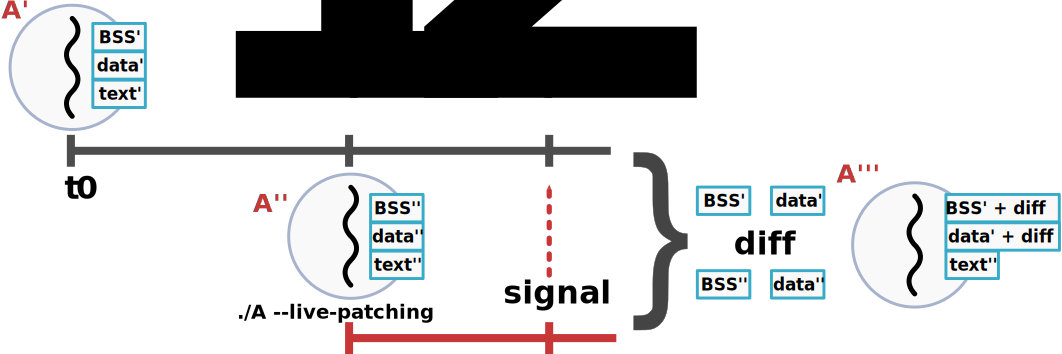
\includegraphics[width=\textwidth]{live-patching}
  \caption{Funcionamento do padrão atualização em tempo de execução}
  \label{fig:atr}
\end{figure}

Buscando uma possível solução para este problema, a Figura~\ref{fig:atr}
ilustra de forma geral o padrão ATE. Na ilustração temos um processo chamado de
$A'$ que é o alvo da atualização em tempo de execução; ainda na figura, repare a linha
do tempo indicando a execução de $A'$. No período de tempo $t_1$, uma instância
idêntica do processo $A$ é iniciada e recebe o nome de $A''$.  Repare que o
processo $A''$ recebe a \emph{flag} \texttt{--live-patching} como parâmetro
durante a sua inicialização, isso significa que $A''$ vai iniciar em um estado
especial; por fim uma fotografia persistente é feita. Quando tal estado é
atingido $A''$ envia um sinal para $A'$, que por sua vez manipula o sinal
recebido.  Dentro da operação de tratamento do sinal, $A'$ faz com que uma
operação de troca (\texttt{BEAD\_SWITCH}) com a \emph{flag} \texttt{DIFF} para
a fotografia de $A''$ aconteça. Essa troca ocorre fazendo uma operação que
calcula a diferença (\emph{diff}) do segmento de \emph{BSS} e \emph{Data} de
$A'$ com $A''$; por fim, é feito uma troca do segmento de texto de $A'$ com
$A''$.

\begin{pseudocode}
\begin{lstlisting}[language=pseudocode, style=pseudocode]
function live_patch_handler(signal)
  // ... qualquer outro tipo de manipulação de sintal ...
  struct bead_data bead

  if signal = SIG_LIVE_PATCHING then
    bead.switch_option $\gets$ DIFF /// \label{line:liveConf}
    \func{beadctl(BEAD_SET_CONFIG, &bead)}

    id $\gets$ \func{get_snapshot_target()} /// \label{line:getSnap}
    \func{beadctl(BEAD_SWITCH, id)}

function live_patch_action()
  // ... qualquer código necessário ...
  \func{persistent_context()}
  \func{signal(SIG_LIVE_PATCHING)}

function MAIN(args) /// \label{line:livePatch}
  if args = "--live-patching" /// \label{line:arg}
    \func{live_patch_action()}
    exit 0
  // ... qualquer código ...
\end{lstlisting}

  \caption{Padrão Atualização em Tempo Real}
  \label{alg:livePatch}
\end{pseudocode}


O Pseudocódigo~\ref{alg:livePatch} ilustra como seria uma possível
implementação do padrão ATE. A função \texttt{MAIN()} de algum programa
qualquer precisaria ser alterada para aceitar o parâmetro
\texttt{--live-patching}\footnote{O nome do parâmetro poderia ser qualquer um
que o programador queira adotar.} como a Linha~\ref{line:arg} ilustra. Se o
parâmetro \texttt{--live-patching} for recebido, uma função especial deve entrar em ação para por o
software em um estado considerado seguro pela aplicação para em seguida tirar
uma fotografia persistente do estado atual; por fim, essa deve enviar um sinal
para o processo que será atualizado. Quando o sinal chegar para a aplicação,
então a função \texttt{live\_patch\_handler()} deve ser executada de forma a
tratar o sinal e como a Linha~\ref{line:liveConf} indica o \emph{bead} deve ser
configurado para realizar a atualização. A Linha~\ref{line:getSnap} mostra uma
função que deve buscar a fotografia persistente referente ao processo, note que
essa função pode ser implementada de várias maneiras visando garantir segurança
e consistência; para esse pseudocódigo, apenas considere que ela retornará o
identificador da fotografia tirada do processo na Linha~\ref{line:arg}. Por
fim, o processo faz a atualização por meio da operação de \texttt{BEAD\_SWITCH}
previamente configurada.

\subsubsection{Padrão Compartimento}
%TODO: Atualizar o switch para ele aceitar os compartimentos. BEAD_CONTEXT_SWITCH -> BEAD_SWITCH

O padrão Compartimento nasce dos conceitos apresentados pelo shred, que busca apresentar uma técnica para evitar ataques intra-processos
baseado em um recurso de hardware subutilizado. Essa ideia é fundamentada em um
novo recurso fornecido por várias CPUs que permite definir domínios de acesso
dentro da memória do processo (Seção~\ref{sec:outros_mecanismos_memoria}). O
principal objetivo do compartimento dentro do próprio processo consiste em
adicionar maior nível de isolamento e dificultar/impedir ataques que ocorram
dentro do processo.

\begin{pseudocode}
\begin{lstlisting}[language=pseudocode, style=pseudocode]
function special_function() /// \label{line:compartimentoFuncaoEsp}
  struct bead_data bead

  bead.compartment_size $\gets 300$
  \func{beadctl(BEAD_SET_CONFIG, &bead)}
  // ... qualquer código que precisa de um bom isolamento ...
  // Aloca memória dentro do compartimento
  \func{beadctl(BEAD_ALLOC_COMPARTMENT_MEMORY, &bead)} /// \label{line:compartimentoAlloc}
  // Libera a memória do compartimento
  \func{beadctl(BEAD_FREE_COMPARTMENT_MEMORY, &bead)} /// \label{line:compartimentoFree}

function enter_compartment()
  struct bead_data bead

  bead.compartments $\gets$ BEAD_ENTER_COMPARTMENT /// \label{line:compartimentoConfig}
  \func{beadctl(BEAD_SET_CONFIG, &bead)}
  \func{beadctl(BEAD_SWITCH, &bead)} // Troca o contexto de executação atual

function exit_compartment() /// \label{line:compartimentoExit}
  struct bead_data bead

  bead.compartments $\gets$ BEAD_EXIT_COMPARTMENT
  \func{beadctl(BEAD_SET_CONFIG, &bead)}
  \func{beadctl(BEAD_SWITCH, &bead)} // Troca o contexto de executação atual

function MAIN() /// \label{line:compartimentoMAIN}
  // ... qualquer código ...
  // Função crítica
  \func{enter_compartment()} /// \label{line:compartimentoEnter}
  \func{special_function()}
  \func{exit_compartment()}
  // ... qualquer código ...
  
\end{lstlisting}

  \caption{Padrão compartimento}
  \label{alg:compartimento}
\end{pseudocode}


O Pseudocódigo~\ref{alg:compartimento} ilustra como esse padrão se comporta. O
exemplo começa na Linha~\ref{line:compartimentoMAIN}, onde a semântica do
código original não sofre alteração. Em um determinado trecho de uma aplicação,
pode ser necessário executar uma operação sobre dados sensíveis (p.ex., senhas),
portanto, é desejável que o acesso a tal informação seja o mais restrito
possível. Nesse contexto, a Linha~\ref{line:compartimentoEnter} ilustra a
operação \texttt{enter\_compartment()} que é responsável por mudar o fluxo de
execução do processo para o compartimento. Em seguida, na
Linha~\ref{line:compartimentoConfig}, podemos acompanhar o processo de
configuração necessário para criar o compartimento. Se tudo ocorrer bem, o processo passa a executar dentro de
um compartimento isolado das demais \emph{threads}. 

A operação \texttt{BEAD\_ENTER\_COMPARTMENT} foi introduzida na Seção~\ref{sec:api}. Ela foi
utilizada no processo de configurar o compartimento e a operação de troca foi
utilizada para entrar em tal modo (vale destacar que esse é um uso diferente da
operação de troca). Dentro do compartimento, não é possível utilizar as operações de alocação de memória
padrão, uma vez que é preciso utilizar o recurso de controle de acesso fornecido
pelo hardware. Nesse sentido, o \emph{bead} fornece a operação
\texttt{BEAD\_ALLOC\_COMPARTMENT\_MEMORY}, responsável por alocar memória e impedindo
a qualquer \emph{thread} externa ter acesso a ela.
A Linha~\ref{line:compartimentoAlloc} é responsável por alocar memória
dentro do próprio compartimento. Por fim, para remover a memória alocada basta
chamar a função \texttt{BEAD\_FREE\_COMPARTMENT\_MEMORY}.

Quando todas as operações sobre dados sensíveis tiver acabado, o programador
pode solicitar ao \emph{bead} para sair do compartimento. A
Linha~\ref{line:compartimentoExit} ilustra a função que faz a operação de sair
do compartimento.

\subsection{A biblioteca \texttt{libbead}}

Na Seção~\ref{sec:padroes}, procuramos evidenciar o comportamento de baixo
nível do \emph{bead} de forma a explicitar o desacoplamento das abstrações de
processos. Na prática, não esperamos que os usuários do \emph{bead} utilizem os
padrões da forma como foi descrito na Seção~\ref{sec:padroes}, uma vez que elas
representam operações de baixo nível. Idealmente, a implementação do
\emph{bead} deve vir acompanhada de uma biblioteca (chamaremos de
\emph{libbead} neste texto) que se comporte como uma camada de abstração sobre
as operações de baixo nível e assim facilite a utilização nos novos recursos
oferecidos pelo \emph{bead}. Note que tal biblioteca deve prover os padrões
descritos da Seção~\ref{sec:padroes}.

O padrão fotografia (Seção~\ref{sec:fotografia}) poderia ser encapsulado em
duas funções: \texttt{beadGetContext()} e \texttt{beadSwitch()}. A função
\texttt{beadGetContext()} espera alguns parâmetro de configuração que definem a
forma como a fotografia deve operar e em seguida salva o contexto.
Posteriormente, o desenvolvedor precisaria realizar o \texttt{beadSwitch()}
para o contexto novo. O Pseudocódigo~\ref{alg:libBeadFotografia} ilustra como
pode ser usado a operação descrita na Seção~\ref{sec:fotografia}, da perpectiva
de um usuário da \emph{libbead}.

\begin{pseudocode}
\begin{lstlisting}[language=pseudocode, style=pseudocode]
function MAIN()
  recursive $\gets$ true
  // ... qualquer código ...
  \func{beadGetContext(recursive, &id)} // Ponto no código no qual é feito uma cópia
  // ... qualquer código ...
  \func{beadSwitch(id)} // Troca o contexto de executação atual
  
\end{lstlisting}

  \caption{\emph{libbead}: Padrão fotografia}
  \label{alg:libBeadFotografia}
\end{pseudocode}


Outra funcionalidade que poderia ser consideravelmente simplificada pela
\texttt{libbead} é a operação de virtualização controlada apresentada na
Seção~\ref{sec:virtctl}. O Código~\ref{alg:libBeadvirtMode} ilustra como a
\texttt{libbead} pode simplificar a tarefa de usar os recursos de
virtualização. Note que a função \texttt{beadVirtualMode()} espera um conjunto
de parâmetros de configuração e uma função para ser executada em modo
virtualização; se \texttt{NULL} for passada no último parâmetro, todo o
processo vai executar em modo de virtualização.

\begin{pseudocode}
\begin{lstlisting}[language=pseudocode, style=pseudocode]
function any_function()
  // ... qualquer código para ser executado em modo virtualização ...      

function MAIN()
  params $\gets$ ALL_VIRT_CAPABILITY
  // ... qualquer código ...
  \func{beadVirtualMode(params, any_function)}
  
\end{lstlisting}

  \caption{\emph{libbead}: Padrão Virtualização Controlada}
  \label{alg:libBeadvirtMode}
\end{pseudocode}


Em termos de utilização do padrão de atualização em tempo de execução
(Seção~\ref{sec:ate}), a \emph{libbead} representa uma enorme simplificação. O
Pseudocódigo~\ref{alg:beadLivePatch} ilustra o padrão ATE da perspectiva do
\emph{libbead}, note que precisamos apenas da função
\texttt{beadInstallLivePatching()} para adicionar suporte para a atualização em
tempo de execução. Essa função instala no processo um mecanismo que leva ele
para um estado \emph{quiescence}~\citep{quiescence} que pode permitir a
atualização em tempo de execução. Note do pseudocódigo, que ainda é necessário
tratar o recebimento do pedido de atualização.

\begin{pseudocode}
\begin{lstlisting}[language=pseudocode, style=pseudocode]
function MAIN(args)
  beadInstallLivePatching()

  if args = "--live-patching"
    \func{live_patch_action()}
    exit 0
  // ... qualquer código ...
\end{lstlisting}

  \caption{\emph{libbead:} Padrão Atualização em Tempo Real}
  \label{alg:beadLivePatch}
\end{pseudocode}


Por fim, o mais importante a se notar sobre a \texttt{libbead} é que ela
comporta-se como uma camada de abstração para as operações de baixo nível. Essa
biblioteca deve tornar simles o processo de utilização do \texttt{bead}, assim
como a \texttt{libc}\footnote{\url{https://www.gnu.org/software/libc/}} e a
\texttt{libdrm}\footnote{\url{https://01.org/linuxgraphics/community/libdrm}}
fazem.

\section{Sumário}

Neste capítulo os nossos objetivos consistiram em responder as seguintes
questões de pesquisa:

\begin{quote}
 \item \textit{QP1:.} ``Quais são as características desejáveis para a próxima geração de abstrações de processos?''
 \item \textit{QP2:.} ``Quais são os principais desafios em se implementar a próxima geração de abstrações de processos?''
\end{quote}

Para responder a primeira questão de pesquisa, fizemos uma análise da
Seção~\ref{sec:extracao} até a \ref{sec:bead} discutindo as diversas
característica desejáveis para a próxima geração de abstração de processos. Em
especial, a Tabela~\ref{tab:desacoplamento_beneficio} apresenta uma visão
centralizada dos diversos desacoplamentos passíveis de serem adotados. Além
disso a Figura~\ref{fig:decomposicao_proc} ilustra graficamente como a nova
geração de abstrações de processo pode se organizar levando-se em consideração
os diversos desacoplamentos sugeridos. Por fim, introduzimos da
Seção~\ref{sec:bead} até \ref{sec:padroes} um modelo teórico chamado de
\emph{bead} que tem por principal objetivo mostrar uma unificação dos diversos
trabalhos e ilustrar os potenciais usos dessa nova técnica.

Para responder a segunda questão de pesquisa, realizamos uma ampla discussão na
Seção~\ref{sec:potenciais} que busca dialogar com o
Capítulo~\ref{cap:validacoes}. Em especial, com base em certos critérios,
criamos a Tabela~\ref{tab:adocao} mostrando o potencial de adoção de novas
abstrações de processos.

Por fim, destacamos que levar avanços para as abstrações de processos atuais
significa abrir novos campos de pesquisa e reaquecer os projetos de SO
modernos. Note que um SO monolítico, como o Kernel Linux, pode mudar
completamente o seu \emph{design} para modelos mais flexíveis e desacoplados
tendo como ponto inicial a evolução dos processos. 

